\documentclass{report}

\usepackage[left=3cm, right=3cm, top=2.5cm, bottom=2.5cm]{geometry}
\usepackage{graphicx}  
\usepackage{bm} 
\usepackage[colorlinks=true]{hyperref}
%\usepackage{lgrind}  
\usepackage{amsmath}
\usepackage{xcolor} 
\usepackage{longtable}    
\usepackage{epsf}         
%\bm{mathsymbol}
\usepackage{asymptote}     
\usepackage{thumbpdf}
\usepackage{booktabs}
\usepackage[italian]{babel}
\usepackage{float}
\usepackage{enumerate}
\usepackage{siunitx}
\usepackage{multicol}
\usepackage{subfigure}
\usepackage{caption}
\usepackage{subcaption}

\usepackage{graphicx}
\usepackage{titlesec}
\usepackage{hyperref}

% Nascondi completamente i numeri di capitolo
\titleformat{\chapter}[display]
  {\normalfont\Huge\bfseries}{}{0pt}{\Huge}

\begin{document}

\begin{titlepage}
    \centering
    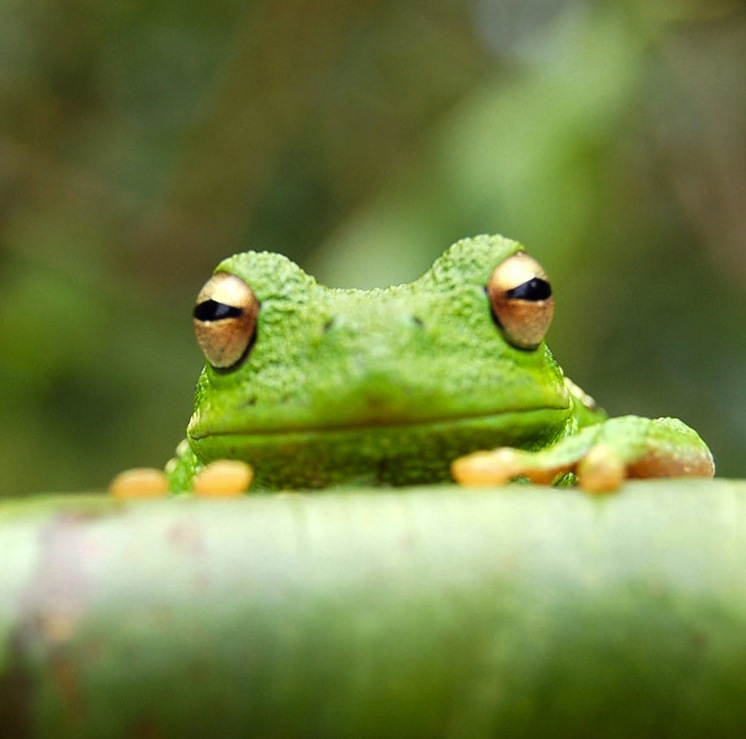
\includegraphics[scale=0.35]{frog.jpg}
    
    \vspace{2cm}
    
    {\huge\textbf{PROGETTO DI RICERCA}}
    
    \vspace{0.5cm}
    
    {\LARGE\textbf{SU PROBLEMI DI NATURA GEOMETRICA}}
    
    \vspace{0.5cm}
    
    {\LARGE\textbf{APPLICABILI AL GIOCO DEL CALCIO}}
    
    \vspace{2cm}
    
    {\Large Luchi Davide, Marcon Giacomo}
    
    \vspace{2cm}
\end{titlepage}

\tableofcontents % Crea l'indice

\chapter{Introduzione e obiettivi}
Il progetto ha come obiettivo quello di rispondere a delle domande di natura geometrica, creando dei modelli applicabili al gioco del calcio. L'idea è quella di partire da una domanda semplice, alla quale nessuno ha mai dato una risposta di natura geometrica, per poi approfondirne lo studio aggiungendo sempre più dettagli e creando un modello che si adatti a diverse situazioni di gioco, in base alle esigenze.\newline
Ma quale è questa domanda? E quali sono i livelli di approssimazione successivi?\newline
\newline
NB: c'è SEMPRE da tenere in considerazione che il calcio è uno sport di \textit{movimento}, e questo progetto tratterà problemi di natura statica, almeno per ora. L'idea è di rispondere a dei quesiti per trarre delle considerazioni generali sull'occupazione del campo, per cercare di capire qualcosa di intrinseco legato a questo sport. Non c'è la presunzione di dettare schemi dinamici, ma solo di capire se ci sono disposizioni statiche più efficienti di altre.\newline
Se dovessero esserci informazioni interessanti, si può pensare di ampliare il progetto in futuro.



\section{Primo step}
"Data una porzione rettangolare (del campo), qual è è la miglior disposizione possibile di dieci cerchi (i giocatori di movimento) in modo da ottimizzare lo spazio occupato?".
\newline
\newline
In primo luogo l'interesse è verificare qual'è lo schema più efficiente per occupare la maggior porzione di terreno utilizzando cerchi di raggio uguale. Questa è una domanda di pura geometria, con probabilemente poca utilità pratica. 

\section{Secondo step}
"Disposizione più precisa, con utilità teorica".
\newline
\newline
Immaginando di dividere il campo in zone più o meno importanti (zona centrale più importante di quella laterale, ad esempio) e vedere qual è la nuova disposizione più efficiente.
Un'idea per capire come dividere il campo è guardare le posizioni medie, attribuendo più 'peso' a determinate zone rispetto che ad altre.


\section{Terzo step}
"Caratterizzare ogni cerchio".\newline
\newline
Dal momento che ogni cerchio rappresenta un giocatore, ogni raggio deve essere modellizzato utilizzando parametri proprie di ogni giocatore, per capire l'area che ognuno può occupare in un determinato intevallo temporale.
Tale intervallo deve essere scelto a priori, e va inteso, ad esempio, come "il tempo entro cui si vuole recuperare il pallone, una volta perso il possesso palla". In base poi a diversi parametri fisici e attitudinali, si deve calcolare il raggio associato a ogni giocatore in quel lasso di tempo.


\section{Quarto step}
"Cambio in base a determinate esigenze".\newline
\newline
Potrebbero esserci dei bisogni come ad esempio il raddoppio su un giocatore avversario particolarmente forte. In questo passaggio alcuni cerchi dovranno intersecarsi in determinate zone del campo.


\end{document}








